\subsection{Постановка задачи на разработку программы}
    Цель работы - реализовать программу скелетной анимации.

\bigskip
Задачи работы:

\smallskip
\begin{my_enumerate}
\item Создание исходных данных (файлов) для скелетной анимации.
\item Загрузка анимации из файла (содержание описанно в ТЗ).
\item Рассчет кадров анимации.
\item Воспроизведение анимации на экране средствами OpenGL.
\item Предоставление пользователю возможности перейти к любому моменту времени в анимации.
\item Отрисовка костей модели.
\item Возможность вкл./выкл. учет нормалей и материалов во время отрисовки.
\item Поддержка двух видов камер в OpenGL. Первый вид это камера, движение которой сковано орбитой вокруг модели, и другой тип это камера двигающаяся совершенно свободно.
\end{my_enumerate}


\subsection{Описание алгоритма и функционирования программы}


%=============================================================
\subsubsection{Выбор алгоритма}

\textbf{Различные подходы}
к созданию программ трех мерной анимации балансируют между методами с большим количеством вычислений и методами, требующими большого объема памяти. Условно можно выделить явные и неявные системы анимации.

\textbf{Явные системы анимации} хранят отдельную модель для каждого кадра.
После записи данных в файл, существует много методов для воспроизведения анимации.
Такие методы требуют лишь элементарной математики.
Однако типичная запись одного трека анимации для одного персонажа занимает около 10MB (в формате MD3).

\begin{figure}[h!]
    \centering
    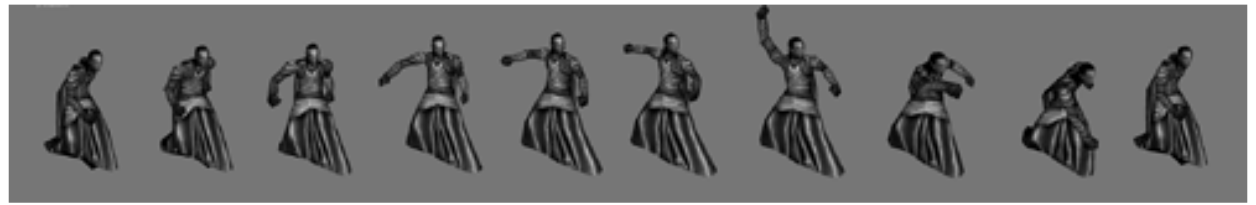
\includegraphics[width=0.8\textwidth]{explicit_animation.png}
    \caption{Каждому кадру соответствует своя модель}
\end{figure}

Предпочтение явным системам отдается, когда необходимо анимировать большие группы людей или животных.

\textbf{Неявные системы анимации} хранят не модели, а более высокоуровневое описание движения.
В частности неявные \textbf{системы скелетной анимации} содержат описание (через матрицу поворота) для каждой кости, как например локоть, плечо, шея.
В реальном времени эти описания применяются к неанимированной модели для расчета следующего кадра анимации.
Эти расчеты требуют более сложной математики и больше времени CPU.


\begin{figure}[h!]
    \centering
    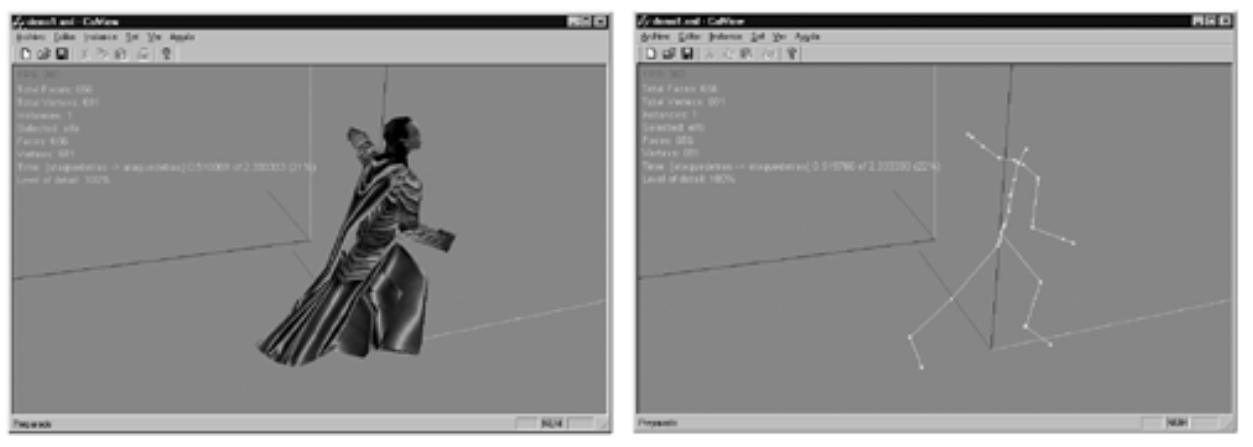
\includegraphics[width=0.8\textwidth]{implicit_animation.png}
    \caption{\small{Слева: анимированный персонаж; справа: скелет для данного кадра}}
    %\label{fig:awesome_image}
\end{figure}

Неявные системы используются, когда персонаж может совершать несколько действий одновременно и невозможно предугадать все возможные варианты анимации.

%=============================================================
\subsubsection{Основные определения и структуры данных}

\textbf{Кость}
Каждая кость содержит информацию о трех мерной трансформации (которая состоит из поворота, растяжения и смещения), а также информацию о кости-отце. Глобальная трансформация кости-потомка, - это произведение глобальной трансформации кости-родителя на локальную трансформацию самой кости-потомка. Изменение транформации родителя, меняет трансформацию потомка.

Ниже приведен класс описывающий кость скелета:
\begin{small}
\begin{verbatim}
class BoneNode
{
    public string Name;
    public Matrix4 GlobalTransform;
    public Matrix4 LocalTransform;

    public BoneNode Parent;
    public List<BoneNode> Children;
    public BoneNode(Node node_data) { ... }
}
\end{verbatim}
\end{small}

\textbf{Скелет}
Скелетом называют иерархичную (дeревообразную) структуру сформированную костями. Скелет определяеться с помощью корневой кости в иерархии.


\textbf{Трек анимации}
В треке содержатся матрицы поворота скелета в ключевые моменты времени.
В упрощенном виде трек можно представить в виде  массива пар: 
$\lbrace$ время ключевого кадра, массив из матриц поворота для каждой кости $\rbrace$

\begin{figure}[h!]
    \centering
    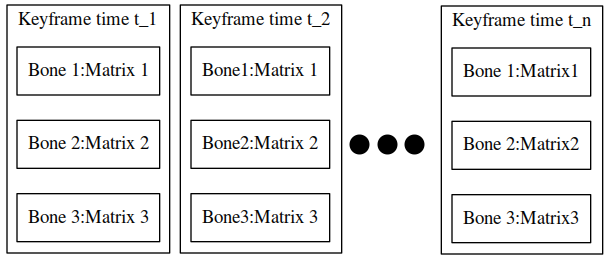
\includegraphics[width=0.4\textwidth]{anim_track.png}
    \caption{\small{В ключевые моменты времени \detokenize{(t_1, t_2, ... t_n)}, каждая кость ставиться в соответствие с матрицей локальной трансформации.}}
    
\end{figure}


\textbf{Модель}
Модель состоит из набора вершин, весов вершин (коэффициентов, определяющих влиение костей на вершину), нормалей, материалов. В пакете для трех мерной анимации модель привязывают к скелету, каждая вершина модели «привязывается» к какой-либо кости скелета (или к нескольким костям). После привязки модели к скелету при движении отдельной кости будут двигаются и все вершины, привязанные к ней.

\begin{figure}[h!]
    \centering
    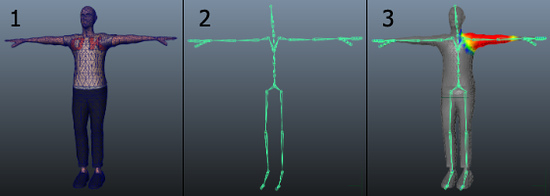
\includegraphics[width=0.6\textwidth]{skinning.png}
    \caption{\small{Слева: модель; в центре: скелет; справа: выделенны вершины модели, которые были привязанны к кости правого предплечья}}
    %\label{fig:awesome_image}
\end{figure}

%=============================================================
\subsubsection{Описание алгоритма}
Для создания эффекта анимации необходимо извлекать из трека набор матриц поворота соответствующий настоящему моменту времени. Применять этот набор матриц к скелету, а затем применять позу скелета к модели (то есть изменять координаты вершин).

\textbf{Применение данных из трека к скелету}
Матрицы поворота для всех костей записываются в треке относительно матрицы поворота родителя.
Поэтому для анимации скелета необходимо применять матрицы в последовательном порядке.
Начинаем с корневой кости и применяем к ней описанную в треке анимации матрицу поворота.
Затем, двигаемся вглубь скелета по иерархии и находим произведение матрицы родителя и матрицы потомка (извлеченной из трека). Другими словами расчитывается глобальная матрица поворота для кости-потомка.

Необходимо продолжать движение по иерархии пока не будут рассмотренны все кости. Ниже приведен псевдокод для применения данных из трека к скелету:

\begin{figure}[h!]
\begin{small}
\begin{verbatim}
deform_skeleton (bone root, matrix global, track matrices)
  get the matrix for root bone from track matrices
  multiply it by matrix global
  store the result in bone root as global transform
  if root has children
    deform (children of this node, root bone global matrix, track matrices)
  end if
end function
\end{verbatim}
\end{small}
\end{figure}

\begin{figure}[h!]
    \centering
    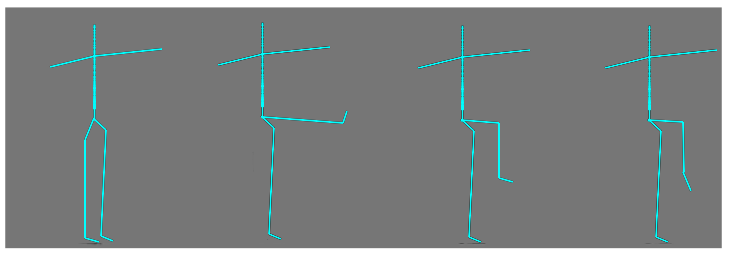
\includegraphics[width=0.6\textwidth]{forward_kinematics_skeleton.png}
    \caption{\small{Последовательное применение преобразований, начиная от копчика (корневой кости) и заканчивая ступней.}}
    %\label{fig:awesome_image}
\end{figure}


\textbf{Применение скелета к модели}

После того как рассчитанны матрицы поворотов для скелета, их необходимо применить на вершины модели.
Для этого используется рекурсивный алгоритм похожий на алгоритм для анимации скелета. Ниже приведен его псевдокод:

\begin{small}
\begin{verbatim}
deform_mesh (bone root, mesh original, mesh deformed)
  for each child_bone of root
    for each vertex in the original mesh
      if bone_weight > 0
          apply bone global transform to vertex
          scale the resulting point by the bone weight
          store the result in deformed
      end if
    end for
    if child_bone has children
      deform_mesh (children of this node, mesh original, deformed)
    end if
  end for
end function
\end{verbatim}
\end{small}

\begin{figure}[h!]
    \centering
    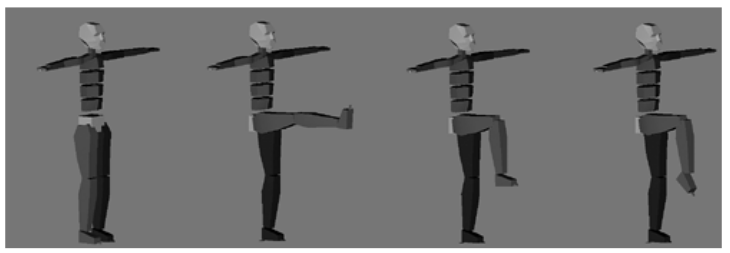
\includegraphics[width=0.8\textwidth]{forward_kinematics.png}
    \caption{\small{Применение преобразований к вершинам модели.}}

\end{figure}



\subsubsection{Реализация программы скелетной анимации}
В программе можно выделить несколько логических блоков. Каждый блок состоит из одного или более классов предоставлающих определенный функционал.

\begin{my_enumerate}
\item Блок чтения данных.
\item Блок хранения состояния анимации.
\item Блок хранения данных модели и скелета.
\item Блок деформации скелета.
\item Блок отрисовки модели.
\item Блок управления компонентами.
\end{my_enumerate}

\textbf{Чтение данных}
С помощью библиотеки Assimp производится чтение из файла. Для оптимальной работы данные перераспределяются из структур Assimp в свои. Другие функции этой библиотеки не используются.
Ниже приведен упрощенный код считывающий информацию из файла и строящий стуктуры данных.

\begin{verbatim}
// функция для загрузки данных из библиотеки Assimp, в созданные структуры данных
public void LoadScene(byte[] filedata)
{
    using (MemoryStream fs = new MemoryStream(filedata))
    {
        _cur_scene = new SceneWrapper(ReadAssimpScene(fs, "dae"));
        // во входных данных всегда только один трек анимации
        _animation_track = _cur_scene.Animations[0];
        // примененает описания из трека анимации к скелету
        _action = new Animator(_animation_track);
        // корневая кость скелета
        BoneNode bones = _cur_scene.BuildBoneNodes("Armature");
        // модель
        Node mesh = _cur_scene.FindNode("Mesh");
        // хранит состояние анимации
        ActionState state = new ActionState();
        // объединет компоненты
        _enttity = new Entity(_cur_scene, mesh, bones, state);
    }
}
\end{verbatim}


\textbf{Хранение состояния анимации}
Класс ActionState хранит состояние анимации. Наиболее важные поля:
\begin{itemize}
\item Трек анимации.
\item Настоящий момент времени в секундах.
\item Массив времени для всех ключевых кадров.
\end{itemize}

Фyнкция SetTime(\dots) используется для перехода к определенному моменту времени. Она находит интервал между ключевыми кадрами, подсчитывает величину интерполяции.

\begin{verbatim}
// функция для прыжка к определенному времени
public void SetTime(double time_seconds)
{            
    double time_ticks = time_seconds * TickPerSec;
    // когда время в секундах переполняеться, запускаем анимацию с начала
    double time = time_ticks % TotalDurationTicks;
    // поиск интервала между ключевыми кадрами
    int start_frame = FindStartFrameAtTime(time_seconds);
    int end_frame = (start_frame + 1) % KeyframeCount;
    // нахождение значения для интерполяции между ключевыми кадрами
    double delta_ticks = KeyframeTimes[end_frame] - KeyframeTimes[start_frame];
    // если необходимо запустить анимацию заново
    if (delta_ticks < 0.0)
    {
        delta_ticks += TotalDurationTicks;
    }
    double blend = (time - KeyframeTimes[start_frame]) / delta_ticks;
    // приписываем результаты расчетов
    OriginKeyframe = start_frame;
    TargetKeyframe = end_frame;
    KfBlend = blend;
}
\end{verbatim}


\textbf{Хранение данных модели и скелета}
Работает со скелетом и моделью.
Реализует функции поиска костей в скелете или подмоделей в модели.
Функция BuildBones строит скелет по данным из модели (скелет как отдельный класс не существует, он определяеться корневой костью).


\textbf{Деформация скелета}
Применяет данные, описывающие (в матрицах поворота) новую позицию для каждой кости к костям из скелета.
То есть деформирует скелет в соответствии с моментом времени в анимации. На вход блока подается класс ActionState, содержащий информацию о состоянии анимации и корневая кость скелета.

\begin{verbatim}
// функция для извлечения матриц поворота из трека и применения их к скелету
public void ChangeLocalFixedDataBlend(ActionState st)
{
    // для каждой кости создает свой канал анимации    
    foreach (NodeAnimationChannel channel in _action.NodeAnimationChannels)
    {
        BoneNode bone_nd = _scene.GetBoneNode(channel.NodeName);
        // поворот кости
        Quaternion target_roto = Quaternion.Identity;
        if (channel.RotationKeyCount > st.TargetKeyframe)
        {
            target_roto = channel.RotationKeys[st.TargetKeyframe].Value.eToOpenTK();
        }
        Quaternion start_frame_roto = channel.RotationKeys[st.OriginKeyframe].Value;
        // интерполяция поворота между двумя ключевыми кадрами
        Quaternion result_roto = Quaternion.Slerp(start_frame_roto, target_roto, (float)st.KfBlend);
        // сдвиг кости
        Vector3 target_trans = Vector3.Zero;
        if (channel.PositionKeyCount > st.TargetKeyframe)
        {
            target_trans = channel.PositionKeys[st.TargetKeyframe].Value;
        }
        Vector3 cur_trans = channel.PositionKeys[st.OriginKeyframe].Value;
        // интерполяция сдвига между двумя ключевыми кадрами
        Vector3 result_trans = cur_trans + Vector3.Multiply(target_trans - cur_trans, (float)st.KfBlend);
        // объединение поворота и сдвига
        Matrix4 result = Matrix4.CreateFromQuaternion(result_roto);
        result.Row3.Xyz = result_trans;
        bone_nd.LocalTransform = result;
    }
}

// функция для расчета глобальной матрицы поворота для каждой кости
// эта матрица будет позднее применена к вершинам модели
private void ReCalculateGlobalTransform(BoneNode nd)
{
    nd.GlobalTransform = nd.LocalTransform * nd.Parent.GlobalTransform;
    foreach (var child in nd.Children)
    {
        ReCalculateGlobalTransform(child);
    }
}
\end{verbatim}



\textbf{Отрисовка модели}
Загружает данные о модели в OpenGL.
Запрашивает OpenGL об выделение буферов памяти под вершины, нормали, цвета вершин и массив индексов. Применяет свойства материала, например: цвет, коэффициент рассеивания света, коэффициент свечения и т.д.

Данные o вершинах, материалах и нормалях необходимо загружать в буферы памяти расположенные на видеокарте для того что бы обеспечить приложению приемлимую скорость отрисовки.
Ниже приведен код для загрузки данных в память видеокарты:

\begin{verbatim}
// объект содержащий идентификационные номера буферов в OpenGL
struct Vbo
{
    public int VertexBufferId;
    public int NormalBufferId;
    public int ElementBufferId;
    public int NumIndices;
}

// функция для создания нового буфера 
// и заполнения его данными из массива векторов
private void NewOpenGLBufferWithFloats(out int outGlBufferId, List<Vector3D> dataBuffer) 
{
    GL.GenBuffers(1, out outGlBufferId);
    GL.BindBuffer(BufferTarget.ArrayBuffer, outGlBufferId);
    int sizeof_vec3d = 12; // X,Y,Z = 3 floats, 4 bytes each
    var byteCount = dataBuffer.Count * sizeof_vec3d;
    var temp = new float[byteCount];
    var n = 0;
    foreach(var v in dataBuffer)
    {
        temp[n++] = v.X;
        temp[n++] = v.Y;
        temp[n++] = v.Z;
    }
    GL.BufferData(BufferTarget.ArrayBuffer, (IntPtr)byteCount, temp, BufferUsageHint.StreamDraw);
    VerifyArrayBufferSize(byteCount);
    GL.BindBuffer(BufferTarget.ArrayBuffer, 0);
}

// функция для загрузки данных о модели в память видеокарты
private void Upload(out Vbo vboToFill)
{
    vboToFill = new Vbo();    
    NewOpenGLBufferWithFloats(out vboToFill.VertexBufferId, _mesh.Vertices);
    if (_mesh.HasNormals)
    {
        NewOpenGLBufferWithFloats(out vboToFill.NormalBufferId, _mesh.Normals);
    }
}

\end{verbatim}

Для создания эффекта движения нeобходимо каждый кадр менять содержимое буферов расположыенных на видеокарте.
А именно необходимо менять координаты вершин и направления нормалей к каждой вершине (для корректного отображения света/тени).
Для этого необходимо послать запрос к драйверу OpenGL и получить указатель на память с загруженными ранее данными.
Далее приведен код модифицирущий данные в буфере для следующего кадра.

\begin{verbatim}
// функция для получения доступа к буферу OpenGL
public void BeginModifyNormalData(out IntPtr data, out int qty_normals)
{
    GL.BindBuffer(BufferTarget.ArrayBuffer, _vbo.NormalBufferId);
    data = GL.MapBuffer(BufferTarget.ArrayBuffer, BufferAccess.ReadWrite);
    qty_normals = _mesh.Normals.Count;
}
// функция для освобождения буфера OpenGL
public void EndModifyNormalData()
{
    bool data_upload_ok = GL.UnmapBuffer(BufferTarget.ArrayBuffer);
    if (! data_upload_ok)
    {
        throw new Exception("OpenGL driver has failed.");
    }
}
\end{verbatim}


\textbf{Управление компонентами}
Класс Entity объединяет компоненты необходимые для анимации одного персонажа. Хранит ссылки на скелет (корневую кость), состояние анимации (ActionState), на саму модель и на класс отрисовки модели (MeshDraw).
    \medskip
    В частности блок персонажа применяет трансформации из скелета к вершинам модели (взвешивая действие каждой кости на вершину) и модифицирует данные в буфере данных OpenGL, что и создает эффект анимации.
    
\begin{verbatim}
// функция в блоке управления компонентами для применения матриц костей к вершинам модели
public void RecursiveTransformVertices(Node node)
{
    foreach (int mesh in nd.Meshes)
    {
        // получаем указатель на буфер в OpenGL
        IntPtr pbuf_opengl;
        int qty_vertices;
        mesh.BeginModifyVertexData(out pbuf_opengl, out qty_vertices);
        // изначальная модель без деформаций
        Mesh original_data = mesh.OriginalData;
        // go over every vertex in the mesh
        unsafe
        {
            int sz = 3;         // размер шага
            float* coords = (float*)pbuf_opengl;
            for (int vertex_id = 0; vertex_id < qty_vertices; vertex_id++)
            {
                Matrix4 matrix_with_offset = mesh._vertex_id2matrix[vertex_id];
                // получить изначальные координаты вершины
                Vector3 vertex_default = original_data.Vertices[vertex_id];
                Vector3 vertex;
                Vector3.Transform(ref vertex_default, ref matrix_with_offset, out vertex);
                // Применение веса к вершине
                Vector3 delta = vertex_default - vertex;
                vertex += delta *  mesh._vertex_id2bone_weight[vertex_id];
                // Запись новых координат обратно в буфер OpenGL
                coords[vertex_id*sz + 0] = vertex.X;
                coords[vertex_id*sz + 1] = vertex.Y;
                coords[vertex_id*sz + 2] = vertex.Z;
            }
        }
        mesh.EndModifyVertexData();

        foreach (Node child in nd.Children)
        {
            RecursiveTransformVertices(child);
        }
    }
}
\end{verbatim}


\subsection{Mетод организации входных и выходных данных}

\subsubsection{Описание метода входных и выходных данных}
Входными данными является файл в формате collada (.dae)
, в котором в обязательном порядке должны присутствовать следующие элементы:
\begin{my_enumerate}
\item Одна полигональная модель.
\item Один трек анимации.
\item Один скелет.
\end{my_enumerate}

Если не выполненны условия на наличие полигональной модели,
трека анимации и связанного с моделью скелета то
у программы не хватит информации для воспроизведения анимации.

Выходными данными является отображение анимации на экране.


\subsection{Выбор состава технических средств}

\subsubsection{Состав технических и програмных средств}
Для возможности запустить приложение необходимо учесть следующие системные требования:
\begin{my_enumerate}
\item Компьютер, оснащенный:
    \begin{my_enumerate}
    \item Обязательно 64-разрядный (x64) процессор с тактовой частотой 1 гигагерц (ГГц) или выше;
    \item 1 ГБ оперативной памяти (ОЗУ);
    \item 1.5 ГБ свободного места на жестком диске;
    \item графическое устройство OpenGL с драйвером версии 3.1 или выше.
    \end{my_enumerate}
\item Монитор
\item Видеокарта
\item Мышь
\item Клавиатура
\end{my_enumerate}
\bigskip

Также необходимо учесть следующие програмные требования:
\begin{my_enumerate}
\item Поддержка OpenGL версии 3.1
\item 64-битная операционная система Windows 7.
\item .NET Framework версии 4.5.1
\item Библиотека Assimp версии 3.1
\item Библиотека OpenTK версии 1.1.4
\end{my_enumerate}

Программа была протестирована и отлажена на версии OS Windows 7 с использованием .Net Framework 4.5.1, OpenTK версии 1.1.4 и Assimp версии 3.1.

Качество и корректность работы программы при других версиях библиотек и операционных систем не проверялось.

Программа использует буферы графической памяти типа STREAM\_WRITE и функции glMapData и glSubBufferData которые в OpenGL официально поддерживаются лишь с версии 3.1

Технические требования к памяти и периферии не превышают технических требований к операционной системе Windows 7 с установленным на ней .Net Framework 4.5.1
